\documentclass{beamer}
\usepackage{amsmath, amssymb, graphicx}
\usepackage{cancel}

\usetheme{Madrid}

\title{Bias-Variance Tradeoff}
\author{Naman Pesricha}
\date{\today}

\begin{document}

\begin{frame}
    \titlepage
\end{frame}

% Slide 1: Notations
\begin{frame}{Notations}
\begin{itemize}
    \item $\mathbf{x}^{(i)}, y^{(i)}$ - $i^{th}$ training input and output pair
    \item $S = \{(\mathbf{x}^{(i)}, y^{(i)})\}_{i=1}^n$ - Training dataset
    \item $\mathcal{D}$ - True population/test distribution
    \item $\mathcal{D}_b$ - Empirical distribution over training set
    
    \item $h^*(\mathbf{x})$ - True underlying function
    \item $\hat{h}_S(\mathbf{x})$ - Model trained on dataset $S$
    \item $h_{\text{avg}}(\mathbf{x}) = \mathbb{E}_S[\hat{h}_S(\mathbf{x})]$ - Average model
    
    \item $\mathbb{E}[\cdot]$ - Expectation operator
    \item $\xi \sim \mathcal{N}(0, \sigma^2)$ - Observation noise
    \item $J(\theta)$ - Training loss function
    \item $L(\theta) = \mathbb{E}_{(\mathbf{x},y)\sim\mathcal{D}}[(y-h_\theta(\mathbf{x}))^2]$ - Population loss
    
    \item $\text{MSE}(\mathbf{x}) = \mathbb{E}_{S,\xi}[(y-\hat{h}_S(\mathbf{x}))^2]$ - Expected test error
\end{itemize}
\end{frame}

% Slide 2: Core Concepts
\begin{frame}{Understanding Generalization}
    $\mathcal{D}_b$: Train/Empirical distribution
    
    $\mathcal{D}$ : Test/True distribution
    \vspace{0.5cm}
    \begin{itemize}
        \item \textbf{GOAL}: Analyze model performance on \textbf{unseen} test examples
        \item \textbf{TRAINING PROCESS}: Minimize loss function $J(\theta)$ on training data $S = \{(x^{(i)}, y^{(i)})\}_{i=1}^n$
        \begin{itemize}
            \item E.g., MSE: $J(\theta) = \frac{1}{n}\sum_{i=1}^n (y^{(i)} - h_\theta(x^{(i)}))^2$
            \item Training data $S$ drawn from empirical distribution $\mathcal{D}_b$
        \end{itemize}
        \item \textbf{TRUE OBJECTIVE}: Minimize \textbf{test error}:
        \[ L(\theta) = \mathbb{E}_{(x,y)\sim\mathcal{D}}[(y - h_\theta(x))^2] \]
    \end{itemize}
\end{frame}

% Slide 3: Practical Considerations
\begin{frame}{Understanding Generalization}
    \begin{block}{Key Takeaway}
         While we minimize training error on $S \sim \mathcal{D}_b$ (train/empirical distribution), our true goal is to perform well on new examples from $\mathcal{D}$ (test/true distribution). \\
        The test examples $(x,y)\sim \mathcal{D}$ are \textbf{unseen} - not used during training.
    \end{block}

    \begin{itemize}
    \item \textbf{In Practice:} We estimate the true test error using a test set
    
    \vspace{0.3cm}
    
    \begin{minipage}{\linewidth}
    \centering
    \begin{tabular}{ll}
    Theoretical: & $L(\theta) = \mathbb{E}_{(x,y)\sim\mathcal{D}}[(y - h_\theta(x))^2]$ \\
    Practical: &  $L(\theta) \approx \widehat{L}(\theta) = \frac{1}{m}\sum\limits_{j=1}^m (y^{(j)}_{\text{test}} - h_\theta(x^{(j)}_{\text{test}}))^2$ \\
    \end{tabular}
    \end{minipage}

    $m$ is the number of examples in the test set.
    
    \vspace{0.3cm}
    
    \begin{itemize}
        \item $\widehat{L}(\theta)$ is our empirical estimate of $L(\theta)$
        \item Requires a sufficiently large, representative test set
        \item Test examples must be \textbf{unseen} during training
    \end{itemize}
\end{itemize}
\end{frame}

\begin{frame}{Understanding Generalization}
    \begin{block}{Generalization Gap}
        The difference between test error and training error is often referred to as the \textbf{generalization gap}.
    \end{block}

    \begin{columns}[T]
        \begin{column}{0.48\textwidth}
            \begin{alertblock}{Overfitting}
                \begin{itemize}
                    \item Small training error ($J(\theta)$)
                    \item Large test error ($L(\theta)$)
                    \item Large generalization gap
                    \item Model fits noise in training data
                \end{itemize}
            \end{alertblock}
        \end{column}
        \begin{column}{0.48\textwidth}
            \begin{alertblock}{Underfitting}
                \begin{itemize}
                    \item Large training error ($J(\theta)$)
                    \item Large test error ($L(\theta)$)
                    \item Small generalization gap
                    \item Model misses true patterns
                \end{itemize}
            \end{alertblock}
        \end{column}
    \end{columns}

    \vspace{0.5cm}
    \footnotesize \textbf{Note}: Even if both train set and test set are sampled from the true distribution $\mathcal{D}$, the test error is not necessarily always close to the training error. As a result, successfully minimizing the training error may not always lead to a small test error.
\end{frame}

\begin{frame}{\underline{\textbf{Intuition}} - Bias and Variance}
    \begin{itemize}
        \item We assume that all true data is generated by a generating function.
        \item While observing the data, we incur some errors:
        \begin{itemize}
            \item Instrumental Error — faulty measuring device
            \item Observation Error — incorrect data reading
            \item Environmental Error — external condition influence
            \item Human Error — mistakes by the observer (I'm looking at you ($\odot \_ \odot$))
            \item Random Errors — unpredictable fluctuations
        \end{itemize}
    \item Defining the following
    \begin{itemize}
        \item $h^*(\mathbf{x})$ or $h^*(x)$ - True underlying function that generates data
        \item $\xi \sim \mathcal{N}(0, \sigma^2)$ - Observation noise (assumed to be Normal)
    \end{itemize}
    \item The actual data we observe is $y = h^*(x) + \xi$ for $(x,y) \sim \mathcal{D}$ 

    \item It's impossible to predict the noise $\xi$, therefore our goal is to essentially recover the function $h^*(x)$
        
    \end{itemize}
\end{frame}

\begin{frame}{\underline{\textbf{Intuition}} - Bias and Variance}
    \begin{center}
        \scriptsize{Train and Test dataset\footnote{\tiny{Diagram: https://cs229.stanford.edu/main\_notes.pdf}}}
        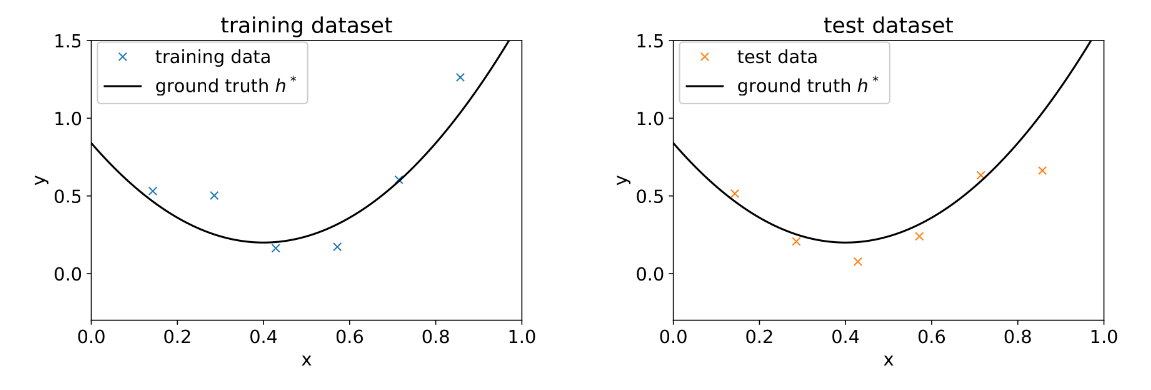
\includegraphics[width=\linewidth]{images/biasvar/TrainAndTest.png} \\
    \end{center}

    \begin{itemize}
        \item We will use the above dataset. The black line represents the true generating function $h^*(x)$ (that we do not observe but wish to model).
        \item The x represents the observed data $y^{(i)} = h^*(x^{(i)}) + \xi^{(i)}$
        \item Note that for the current example, $h^*(x)$ is a quadratic function.
    \end{itemize}
\end{frame}

\begin{frame}{Intuition - \underline{\textbf{Bias}} and Variance}
    \begin{center}
                \scriptsize{Fitting a linear model to a quadratic data\footnote{\tiny{Diagram: https://cs229.stanford.edu/main\_notes.pdf}}}
        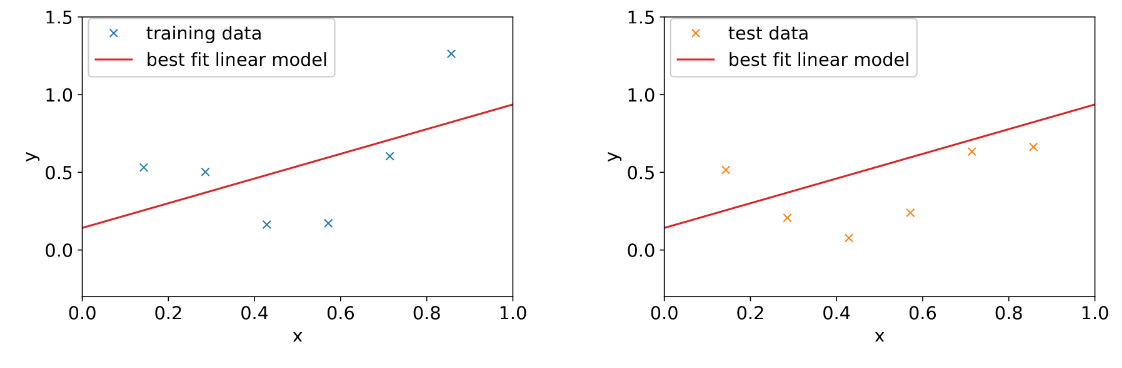
\includegraphics[width=\linewidth]{images/biasvar/BiasTrainAndTest.png}
    \end{center}
    \begin{itemize}
        \item The best fit linear model cannot predict target $y$ from $x$.
        \item This is because the true nature of the relationship between $y$ and $x$ is not linear but is a more complex function.
        \item We cannot expect a linear model to capture $h^*(x)$, which is more complex.
    \end{itemize}
    
\end{frame}

\begin{frame}{Intuition - \underline{\textbf{Bias}} and Variance}
    \begin{center}
                \scriptsize{\footnote{\tiny{Diagram: https://cs229.stanford.edu/main\_notes.pdf}}}
        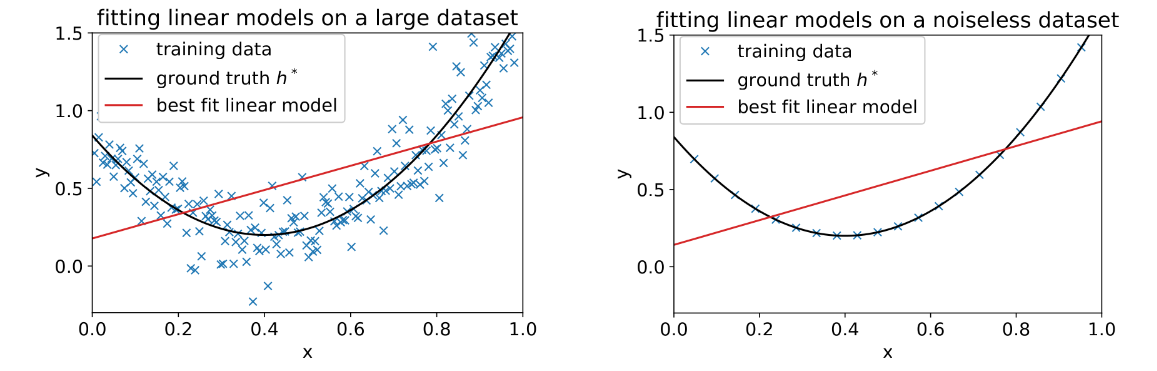
\includegraphics[width=\linewidth]{images/biasvar/biasLargeAndNoiseless.png}
    \end{center}
    \begin{itemize}
        \item This issue cannot be mitigated with  large amount of training samples (even infinite examples), the best fitted linear model will fail to capture the structure of the data.
        \item Even having noiseless data $\xi = 0$, the linear model will still fail.
    \end{itemize}
\end{frame}

\begin{frame}{Intuition - \underline{\textbf{Bias}} and Variance}
    \begin{block}{Informal Definition: \textbf{Bias}}
        The bias of a model is the test error that we get when we fit to a very (say, infinitely) large training dataset
    \end{block}

    \textbf{Takeaways}
    
    \begin{itemize}
        \item The fundamental bottleneck here is the simple model's (Linear in our case) inability to capture the structure in data (quadratic in our case).
        \item The lack of data is not the bottleneck here, and increasing training samples will not help mitigate the problem.
        \item We will need to increase the complexity of the model hoping that the complex model will be able to capture the complex structures in the data.
    \end{itemize}
\end{frame}

\begin{frame}{Intuition - Bias and \underline{\textbf{Variance}}}
    \begin{center}
        \scriptsize{Fitting a 5th degree model to quadratic data \footnote{\tiny{Diagram: https://cs229.stanford.edu/main\_notes.pdf}}}
        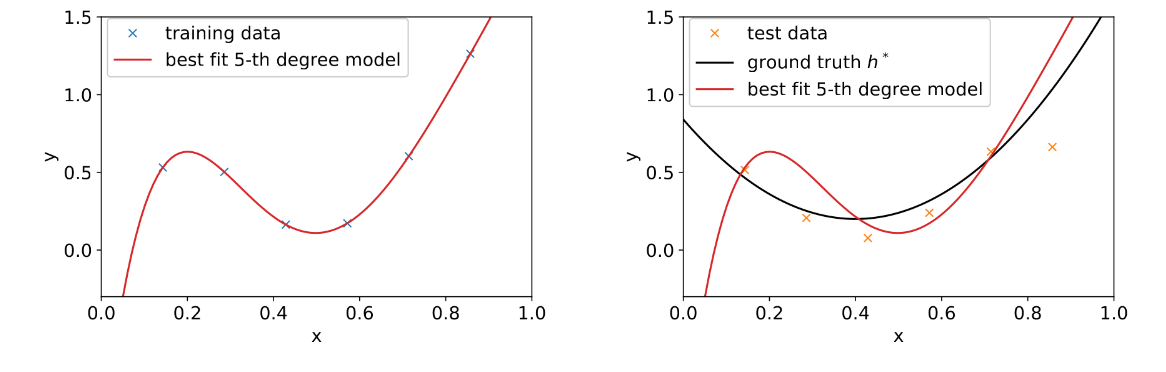
\includegraphics[width=\linewidth]{images/biasvar/5D_on_small.png}
    \end{center}

    \begin{itemize}
        \item The learnt 5th degree model works well on training data but fails to generalize on test data.
        \item The model gives very less error on training samples but very high error on test samples — large generalization gap.
    \end{itemize}
\end{frame}

\begin{frame}{Intuition - Bias and \underline{\textbf{Variance}}}
    \begin{center}
        \scriptsize{\footnote{\tiny{Diagram: https://cs229.stanford.edu/main\_notes.pdf}}}
        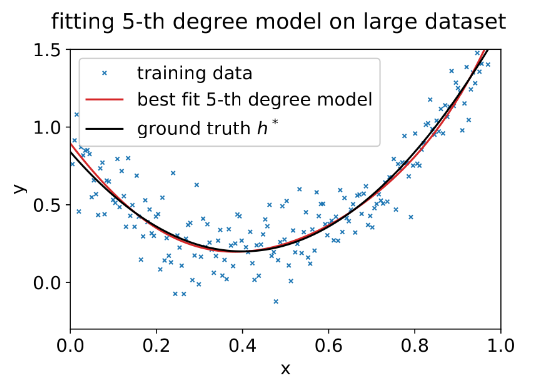
\includegraphics[width=0.4\linewidth]{images/biasvar/5D_on_Large.png}
    \end{center}

    \begin{itemize}
        \item Contrary to behaviour of simple models (Linear in our case), complex (5th degree model) exhibits low bias.
        \item From the diagram, we can see that the model learns the nature of $h^*(x)$ for larger datasets.
        \item The failure can be captured by the \textbf{variance} component of the test error.
    \end{itemize} 
\end{frame}

\begin{frame}{Intuition - Bias and \underline{\textbf{Variance}}}
    \begin{block}{Informal Definition: \textbf{Variance}}
        The variance of a model is the test error that arises because the model is too sensitive to the specific patterns in a finite training dataset.
    \end{block}

    \textbf{Takeaways}
    
    \begin{itemize}
        \item The fundamental bottleneck here is the complex model's tendency to fit spurious patterns (due to noise) in the small training data.
        \item The small and noisy training set makes the model overfit, learning noise rather than patterns, and hence doesn’t generalize well.
        \item We will need to regularize the model or reduce its complexity to mitigate overfitting and improve generalization.
        \item Adding more data will help mitigate the problem of Variance.
    \end{itemize}
\end{frame}

\begin{frame}{Intuition - Bias and \underline{\textbf{Variance}}}
    \begin{center}
        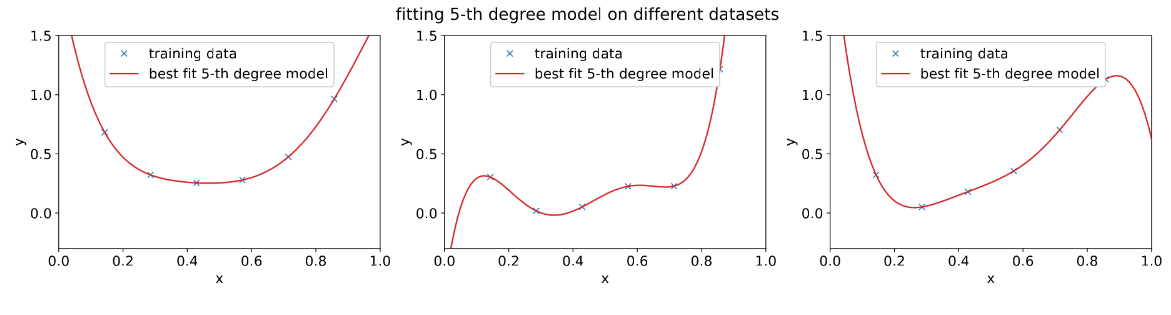
\includegraphics[width=\linewidth]{images/biasvar/5DonDiffData.png} \\
        \scriptsize{Models overfitting different datasets}
    \end{center}

    \vspace{0.3cm}

    \begin{itemize}
        \item Variance measures how models vary across different training datasets (drawn from the same underlying distribution).
        \item Each dataset contains different “spurious patterns” due to noise and input randomness.
        \item Overfitting to dataset-specific patterns causes models to differ greatly.
        \item Models trained on different datasets are highly dissimilar when variance is high.
    \end{itemize}
\end{frame}

\begin{frame}{Bias-Variance Tradeoff}
    \begin{center}
        \scriptsize{Typical bias-variance tradeoff curve \footnote{\tiny{Diagram: https://cs229.stanford.edu/main\_notes.pdf}}}
        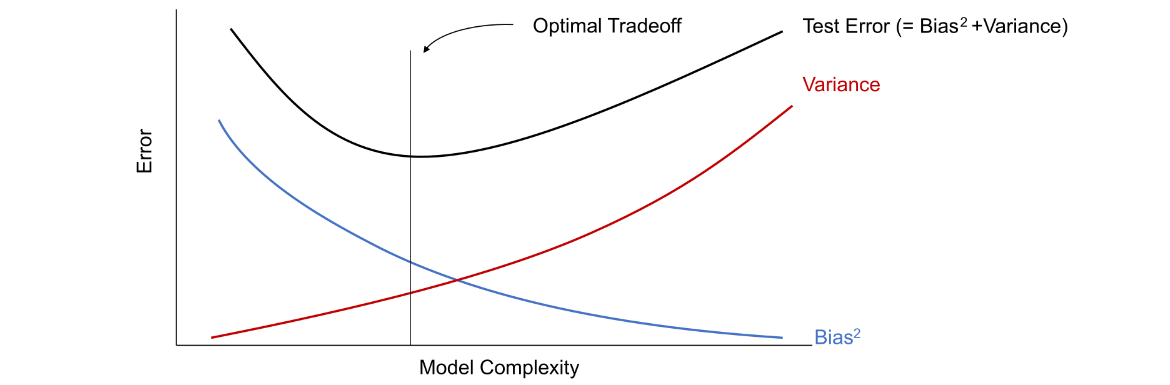
\includegraphics[width=0.7\linewidth]{images/biasvar/biasVarianceTradeoff.png} \\
    \end{center}


    \begin{itemize}
        \item There is often a tradeoff between bias and variance.
        \item \textbf{Simple models} (few parameters) have high bias and low variance → underfitting.
        \item \textbf{Complex models} (many parameters) have low bias and high variance → overfitting.
        \item The goal is to balance bias and variance for optimal generalization.
    \end{itemize}
\end{frame}

\begin{frame}{Good Fit Model}
    \begin{center}
        \scriptsize{A model with a good bias-variance tradeoff \footnote{\tiny{Diagram: https://cs229.stanford.edu/main\_notes.pdf}}}
        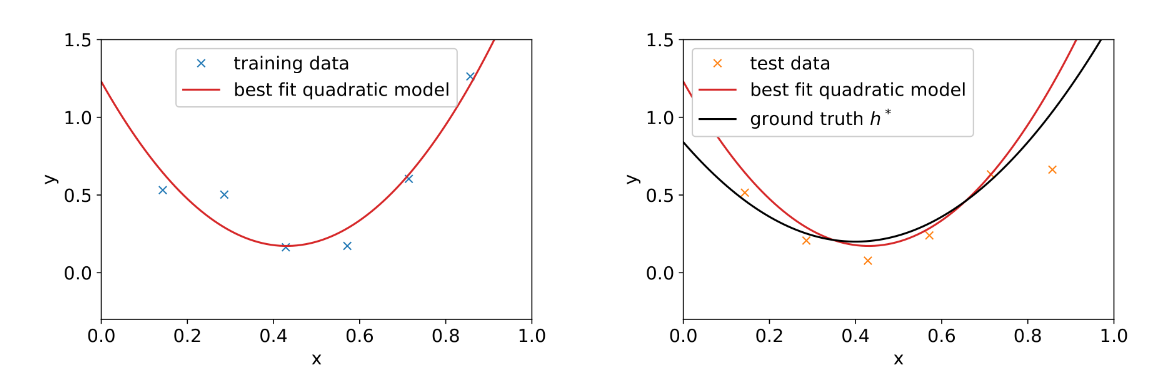
\includegraphics[width=1\linewidth]{images/biasvar/goodfit.png} \\
    \end{center}

    \begin{itemize}
        \item A good fit model balances bias and variance effectively.
        \item The quadratic model achieves low training and test error.
        \item In practice we should tune the model complexity to achieve the best tradeoff.
    \end{itemize}
\end{frame}

\begin{frame}{Mathematical Decomposition for Regression}

    Consider a supervised learning setting with dataset and noise defined as follows:
    \vspace{0.3cm}
    \begin{itemize}
        \item Draw a training dataset $S = \{(x^{(i)}, y^{(i)})\}_{i=1}^n$ where:
        \[
        y^{(i)} = h^*(x^{(i)}) + \xi^{(i)}, \quad \xi^{(i)} \sim \mathcal{N}(0, \sigma^2)
        \]
        
        \item Train a model $\hat{h}_S$ on the dataset $S$.

        \item Take a test example $(x, y)\sim\mathcal{D}$ where:
        \[
        y = h^*(x) + \xi, \quad \xi \sim \mathcal{N}(0, \sigma^2)
        \]

        \item Measure the expected test error (averaged over random draws of $S$ and $\xi$):
        \[
        \text{MSE}(x) = \mathbb{E}_{S, \xi} \left[ (y - \hat{h}_S(x))^2 \right]
        \]
    \end{itemize}
\end{frame}

\begin{frame}{Mathematical Decomposition for Regression}
    \scriptsize{
        $\text{MSE}(x) = \mathbb{E}_{S, \xi} \left[ (y - \hat{h}_S(x))^2 \right]$ \hfill 
    
        \hspace{1cm} $= \mathbb{E}_{S, \xi} \left[ (h^*(x) + \xi - \hat{h}_S(x))^2 \right]$ \hfill \{using $y = h^*(x) + \xi$\} \hspace{0.2cm}
    
        \hspace{1cm} $= \mathbb{E}_{S, \xi} \left[ (h^*(x) - \hat{h}_S(x) + \xi)^2 \right]$ \hfill \{ Rearranging \} \hspace{0.2cm}
    
        \begin{center}
            \{ Expanding the square\} 
        \end{center}  
    
        \hspace{1cm} $= \mathbb{E}_S \left[ (h^*(x) - \hat{h}_S(x))^2 \right] + 2 \cdot \mathbb{E}_{S, \xi} \left[ (h^*(x) - \hat{h}_S(x))  \cdot \xi \right] + \mathbb{E}[\xi^2]$ 
    
        \begin{center}
            \{ $\mathbb{E}[AB] = \mathbb{E}[A]\mathbb{E}[B]$ if $A$ and $B$ are independent \}
        \end{center} 
        
        \hspace{1cm} $= \mathbb{E}_S \left[ (h^*(x) - \hat{h}_S(x))^2 \right] + 2 \cdot \mathbb{E}_S \left[ (h^*(x) - \hat{h}_S(x)) \right] \cdot \mathbb{E}[\xi] + \mathbb{E}[\xi^2]$ 
    
        \begin{center}
            \{ $\xi \sim \mathcal{N}(0, \sigma^2) \implies \mathbb{E}[\xi] = 0 \text{ and } \mathbb{E}[\xi] = \sigma^2$ \}
        \end{center} 
        
        \hspace{1cm} = $\mathbb{E}_S \left[ (h^*(x) - \hat{h}_S(x))^2 \right]  + \sigma^2$ \hfill \{$\bigstar$\} \hspace{0.2cm}
    }
    
\end{frame}


\begin{frame}{Mathematical Decomposition for Regression}
    \begin{itemize}
        \item Define the \textbf{average model}: $h_{\text{avg}}(x) = \mathbb{E}_S [\hat{h}_S(x)]$
        \item $h_{\text{avg}}$ is the prediction averaged over models trained on infinitely many datasets.
        \item It is a hypothetical model (cannot be obtained in practice).
        \item In many cases, $h_{\text{avg}}$ approximates the model trained on a single dataset with infinite samples.
        \item Provides an intuitive interpretation of \textbf{bias}.
    \end{itemize}

    We can decompose the 1st term of  $\text{MSE}(x) =\mathbb{E}_S \left[ (h^*(x) - \hat{h}_S(x))^2 \right]  + \sigma^2$ as follows:

    \[
        \boxed{(h^*(x) - \hat{h}_S(x))^2 = [(h^*(x) - h_{\text{avg}}(x)) +  (h_{\text{avg}}(x) - \hat{h}_S(x))]^2}
    \]
    \[
        C =h^*(x) - h_{\text{avg}}(x) \text{ and } A = h_{\text{avg}}(x) - \hat{h}_S(x)
    \]

    We will abuse $\mathbb{E}[C^2] = C^2$ and $\mathbb{E}[A]=0 $ later.
\end{frame}


\begin{frame}{Mathematical Decomposition for Regression}

\scriptsize{
    Continuing from \{$\bigstar$\}
    
    $\text{MSE}(x) = \mathbb{E}_S \left[ (h^*(x) - \hat{h}_S(x))^2 \right]  + \sigma^2$ \hfill \{$\bigstar$\}

    \vspace{0.2cm}

    \begin{center}
        \{ using $C = h^*(x) - h_{\text{avg}}(x)$ and $A = h_{\text{avg}}(x) - \hat{h}_S(x)$ \}
    \end{center} 

    \vspace{0.2cm}

    $\text{MSE}(x) = \mathbb{E}_S \left[ (C + A)^2 \right] + \sigma^2$  \hfill \{expand square\}

    \vspace{0.2cm}

    \hspace{1cm} $= \mathbb{E}_S[C^2] + \mathbb{E}_S[A^2] + 2 \cdot \mathbb{E}_S[CA] + \sigma^2$

    \vspace{0.2cm}

    \hspace{1cm} $= C^2 + \mathbb{E}_S [A^2] + 2C \cdot \mathbb{E}_S [A] + \sigma^2$ \hfill \{since $C$ is constant $\Rightarrow \mathbb{E}_S[C]=C$\}

    \vspace{0.2cm}

    \hspace{1cm} $= C^2 + \mathbb{E}_S [A^2] + \sigma^2$ \hfill \{since $\mathbb{E}_S[A] = 0$\}

    \vspace{0.2cm}

    \hspace{1cm} $= (h^*(x) - h_{\text{avg}}(x))^2 + \mathbb{E}_S \left[ (h_{\text{avg}}(x) - \hat{h}_S(x))^2 \right] + \sigma^2$ 

    \vspace{0.2cm}

    Final decomposition:

    \[
    \boxed{ \text{MSE}(x) = \underbrace{ \sigma^2 }_{\text{Noise}} + \underbrace{ (h^*(x) - h_{\text{avg}}(x))^2 }_{\text{Bias}^2} + \underbrace{ \mathbb{E}_S \left[ (h_{\text{avg}}(x) - \hat{h}_S(x))^2 \right] }_{\text{Variance}} }
    \]

}

\end{frame}

\begin{frame}{Mathematical Decomposition for Regression}

    \[
    \boxed{ \text{MSE}(x) = \underbrace{ \sigma^2 }_{\text{Noise}} + \underbrace{ (h^*(x) - h_{\text{avg}}(x))^2 }_{\text{Bias}^2} + \underbrace{ \mathbb{E}_S \left[ (h_{\text{avg}}(x) - \hat{h}_S(x))^2 \right] }_{\text{Variance}} }
    \]

    \small
    \begin{itemize}
        \item \textbf{Bias term (squared)}  
        \begin{itemize}
            \item Captures error due to lack of expressivity in the model class.
            \item Even with infinite data, the model family cannot approximate the true function $h^*$.
            \item Example: Linear models cannot approximate a quadratic $h^*$, so bias remains large.
        \end{itemize}
    
        \vspace{0.2cm}
    
        \item \textbf{Variance term}  
        \begin{itemize}
            \item Captures error due to sensitivity of the learned model to randomness in the dataset.
            \item Measures how much $\hat{h}_S(x)$ fluctuates across different datasets.
            \item Often decreases as dataset size increases.
        \end{itemize}
    
        \vspace{0.2cm}
    \end{itemize}

\end{frame}

\begin{frame}{Mathematical Decomposition for Regression}

    \[
    \boxed{ \text{MSE}(x) = \underbrace{ \sigma^2 }_{\text{Noise}} + \underbrace{ (h^*(x) - h_{\text{avg}}(x))^2 }_{\text{Bias}^2} + \underbrace{ \mathbb{E}_S \left[ (h_{\text{avg}}(x) - \hat{h}_S(x))^2 \right] }_{\text{Variance}} }
    \]

    \small
    \begin{itemize}
        \item \textbf{Noise term} ($\sigma^2$)  
        \begin{itemize}
            \item Represents irreducible error from inherent randomness (noise) in data.
            \item Cannot be eliminated as noise $\xi$ is unpredictable by definition.
        \end{itemize}
    \end{itemize}

\end{frame}

\begin{frame}{}
    \LARGE \centering \textbf{Bonus Topic} \\ The Double Descent Phenomenon
\end{frame}

\begin{frame}{The Double Descent Phenomenon}
    \begin{center}
        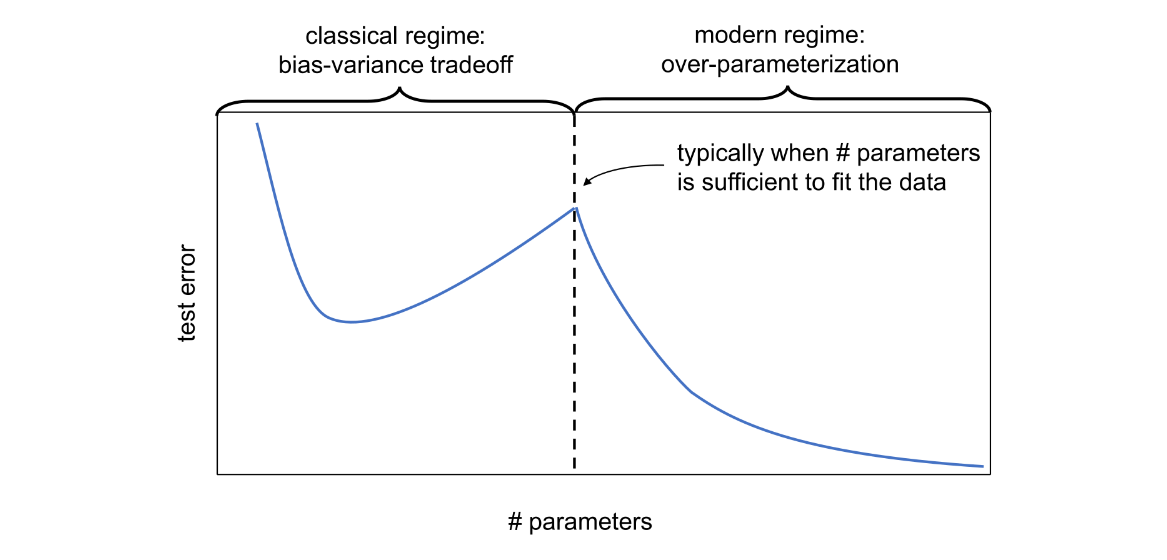
\includegraphics[width=0.7\linewidth]{images/biasvar/DoubleDescent.png} \\
        \scriptsize{Test error vs. model complexity (Double Descent curve)\footnote{\tiny{Diagram: https://cs229.stanford.edu/main\_notes.pdf}}}
    \end{center}

    \begin{itemize}
        \item The tradeoff curves don't follow the convex shape when the model complexity is simply measured by the number of parameters. 
        \item Test error first decreases, then increases, and finally decreases again as model complexity increases.     
    \end{itemize}
\end{frame}

\begin{frame}{The Double Descent Phenomenon}
    \begin{itemize}
        \item The second descent appears in the overparameterized regime, where the number of parameters exceeds the number of data points.
        \item Observed typically in deep neural networks.
        \item Overparameterized models can outperform all simpler models by achieving lower test error.
        \item Scaling to large models can improve test performance beyond the first error minimum.
        \item The phenomenon encourages experimenting with large models instead of fearing overfitting.
        \item In many cases, larger overparameterized models consistently lead to better test performance without a second ascent.
    \end{itemize}
\end{frame}

\begin{frame}{}
    \LARGE \centering \textbf{Thank You }
\end{frame}


\end{document}
